\documentclass[11pt,reqno]{amsart}
\usepackage[top=1in, left=1in, right=1in, bottom=1in]{geometry}                
\geometry{letterpaper}                   % ... or a4paper or a5paper or ...

\usepackage[parfill]{parskip}    % Activate to begin paragraphs with an empty line rather than an indent
\usepackage{algorithm}
\usepackage{algpseudocode}
\usepackage{hyperref}
\usepackage{url}
\usepackage{verbatim}
\usepackage{amssymb}
\usepackage{amsmath}
\usepackage{enumitem}
\usepackage{setspace}
\usepackage{natbib}
\usepackage{algpseudocode}
\usepackage{graphicx}
\usepackage{times}

%\usepackage{epstopdf}
%\DeclareGraphicsRule{.tif}{png}{.png}{`convert #1 `dirname #1`/`basename #1 .tif`.png}

\newcommand{\RR}{I\!\!R} %real numbers
\DeclareMathOperator{\diag}{diag}

\algnewcommand{\Inputs}[1]{%
  \State \textbf{Inputs:}
  \Statex \hspace*{\algorithmicindent}\parbox[t]{.8\linewidth}{\raggedright #1}
}
\algnewcommand{\Initialize}[1]{%
  \State \textbf{Initialize:}
  \Statex \hspace*{\algorithmicindent}\parbox[t]{.8\linewidth}{\raggedright #1}
}

\title[]{An Ultra-sensitive variant detection model using Bayesian variational inference for heterogeneous next-generation sequencing data}
\author{Fan Zhang, Patrick Flaherty}
%Department of Biomedical Engineering, Worcester Polytechnic Institute, Worcester, MA, USA,\\
%Department of Mathematics and Statistics, University of Massachusetts, Amherst, MA, USA}

\begin{document}

\maketitle

\begin{abstract}
The detection of rare variants is significant to capture heterogeneity in clinical populations.
Recently, next-generation sequencing (NGS) technologies have enabled the identification of single nucleotide variants (SNVs) in mixed samples.
Yet, an accurate statistical method is still required to characterize genomic heterogeneity to interrogate the biological causes at the single nucleotide level.
We propose a novel Bayesian statistical model and a variational expectation-maximization (EM) algorithm to estimate variant allele frequency (VAF) and identify SNVs in heterogeneous cell populations.
We demonstrate that our variational algorithm has higher sensitivity and specificity than Markov Chain Monte Carlo (MCMC) sampling method for detecting rare variants with 0.1\% VAF in a synthetic data set,
and is more computationally efficient on tests of low coverage (27$\times$ and 298$\times$) synthetic data.
We show that our model with variational EM inference has higher specificity than some state-of-the-art algorithms.
In an analysis of a directed longitudinal yeast data set, we are able to identify time-series trend in variant allele frequency and detect novel variants that have not yet been reported.
Our model also detects the emergence of a beneficial variant earlier than was previously shown, and a pair of concomitant variants in an independent experiment.
\end{abstract}

\section{Introduction}
%%%%%%%%%%%%%%%%%%%%%%%%%%%%%%%%%%%%%%%%%%%%%%%%%%%%%%%%%%%%%% Motivation %%%%%%%%%%%%%%%%%%%%%%%%%%%%%%%%%%%%%%%%%%%%%%%%%%%%%%%%%%%%%%%%%%
Massively parallel sequencing data generated by next-generation (NGS) technologies is routinely used to interrogate single nucleotide variants (SNVs) in research samples \citep{koboldt2013next}.
For example, deep sequencing shows that HIV infection and influenza may genetically heterogeneous within sub-populations \citep{flaherty2011ultrasensitive}.
Many solid tumors are represented as having intra-tumor heterogeneity by DNA sequencing technology, where SNVs are rare in the population \citep{navin2010inferring}.
Also, whole genome sequencing has revealed that many beneficial mutations of minor allele frequencies are essential to respond to dynamic environments \citep{kvitek2013whole}.
However, rare SNVs identification in heterogeneous cell populations is challenging, because an effective variant detection method is still required due to the intrinsic error rate of next generation sequencing platform \citep{shendure2008next}.
Thus, there is a need for accurate and scalable statistical methods to uncover SNVs in heterogeneous samples.
With the help of computational methods, we are able to detect rare SNVs that will enable a better application of genetic diseases diagnostics.

%%%%%%%%%%%%%%%%%%%%%%%%%%%%%%%%%%%%%%%%%%%%%%%%%%%%%%%%%%%%%%%%%% Classes of Methods %%%%%%%%%%%%%%%%%%%%%%%%%%%%%%%%%%%%%%%%%%%%%%%%%%%%%%%
%%%%%%%%%%%%%%%%%%%%%%%%%%%%%%%%%%%%%%%%%%%%%%%%%%%%%%%%%%%%%%%%%% Probabilistic methods: Bayesian %%%%%%%%%%%%%%%%%%%%%%%%%%%%%%%%%%%%%%%%%%
A number of computational methods are being developed to detect SNVs in large scale genomic data sets.
Among all of the current probabilistic methods, the Bayesian probabilistic framework has been increasingly used to calculate the unobserved quantities such as variant allele frequency given the observed genomic sequencing data.
GATK \citep{mckenna2010genome} and SAMTools \citep{li2009sequence} use a naive Bayesian decision rule to call variants;
However, they fail to call true rare variants in mixed samples \citep{he2015rvd2}.
A major challenge is to distinguish true variants from sequencing errors in order to detect rare variants in heterogeneous samples.
To overcome this problem, we developed an empirical Bayesian hierarchical model with a rare variant detection (RVD) algorithm to characterize a null hypothesis error rate distribution at each position using Beta-Binomial model to fit the reference sequence data. Using this, we call rare variants by comparing the error rate of the sample sequence data to the null distribution \citep{flaherty2011ultrasensitive}.
RVD can identify mutant positions at a 0.1\% fraction in mixed samples using high read depth data.
EBCall is another empirical Bayesian mutation calling method that models sequencing errors based on a Beta-Binomial distribution, where the parameters and latent variables are estimated from a set of non-paired normal sequencing samples \citep{shiraishi2013empirical}.
EBCall is able to accurately call a variant with $<$10\% VAF within heterogeneous samples, but moderate-to-high allele frequencies are required.
Similarly to EBCall, CRISP considers multiple signals to obtain sequencing errors by evaluating the probability of multiple non-reference sequences \citep{bansal2010statistical}.
However, the bottleneck of CRISP is its low computational efficiency due to a calculation of a large amount of contingency tables.
% Other Bayesian methods: MAQ, Mutect, and FamSeq

%%%%%%%%%%%%%%%%%%%%%%%%%%%%%%%%%%%%%%%%%%%%%%%%%%%%%%%%%%%%%%%%%%%%% Joint distribution %%%%%%%%%%%%%%%%%%%%%%%%%%%%%%%%%%%%%%%%%%%%%%%%%%%%%
The above methods test a variant by comparing the sequencing data sets between a matched tumour and normal pair.
In contrast to independently analyzing tumour-normal data sets, JointSNVMix introduces two Bayesian probabilistic models to jointly analyze a tumour-normal paired allelic count of NGS data \citep{roth2012jointsnvmix}.
JointSNVMix derives an expectation maximization (EM) algorithm to calculate $\mathit{maximum} \mathit{a} \mathit{posteriori}$ (MAP) to approximate latent variables in the probabilistic graphical model.
Additionally, Strelka \citep{saunders2012strelka} and SomaticSniper \citep{larson2012somaticsniper} are built to model the joint probabilistic distribution and then call variants in analyzing tumour-normal paired sequence data.

%%%%%%%%%%%%%%%%%%%%%%%%%%%%%%%%%%%%%%%%%%%%%%%%%%%%%%%%%%%%%%%%%%%%%% Frequentist %%%%%%%%%%%%%%%%%%%%%%%%%%%%%%%%%%%%%%%%%%%%%%%%%%%%%%%%%%%%
As an alternative to Bayesian methods, SNVer focuses on a frequentist method that is able to calclate $P$-values, but as a frequentist approach it fails to model sampling bias and error that will reduce the power of detecting true rare variants \citep{wei2011snver}.
Furthermore, Roth, $\mathit{et} \mathit{al}$, compares the performance of two frequentist statistical methods (independent Fisher and joint Fisher) with JointSNVMix.
This work reveals that Fisher methods have lower specificity than JointSNVMix, a Bayesian probabilistic framework \citep{roth2012jointsnvmix}.
%%%%%%%%%%%%%%%%%%%%%%%%%%%%%%%%%%%%%%%%%%%%%%%%%%%%%%%%%%%%%%%%%% Heuristic %%%%%%%%%%%%%%%%%%%%%%%%%%%%%%%%%%%%%%%%%%%%%%%%%%%%%%%%%%%%%%%%%%
An alternative strategy to a probabilistic method is a heuristic method, which is performed by satisfying a set of criteria instead of modeling probabilistic distributions.
%By setting thresholds of the rules, heuristic algorithms can find a good solution, but optimum is not guaranteed.
VarScan is an example of a heuristic method that compares between tumor and normal samples by satisfying some lower bounds, such as a certain variant allele frequency and a number of allele counts \citep{koboldt2012varscan}.
%VarScan is based on Fisher's exact test to estimate sample allele frequencies.

%%%%%%%%%%%%%%%%%%%%%%%%%%%%%%%%%%%%%%%%%%%%%%%%%%%%%%%%%%%%%%%%%% RVD2 %%%%%%%%%%%%%%%%%%%%%%%%%%%%%%%%%%%%%%%%%%%%%%%%%%%%%%%%%%%%%%%%%%%%%%%%
We previously developed a hierarchical Bayesian model, RVD2, to estimate VAF and call SNVs in heterogeneous samples from NGS data \citep{he2015rvd2}.
In RVD2, we derived a Markov Chain Monte Carlo (MCMC) sampling algorithm for posterior inference.
However, the main limitation of MCMC is that it is hard to diagnose convergence and handle nonconjugate events \citep{jordan1999introduction}.
An alternative method is to use variational inference, which is based on a proposed variational distribution over latent variables \citep{jordan1999introduction}.
By optimizing variational parameters, it is potential to acquire an approximate distribution that is close to the true posterior distribution.
Variational inference is also more accurate to handle nonconjugate distributions and more efficient than MCMC sampling \citep{peterson1989explorations}.

%%%%%%%%%%%%%%%%%%%%%%%%%%%%%%%%%%%%%%%%%%%%%%%%%%%%%%%%%%%%%%%%%% RVD3 %%%%%%%%%%%%%%%%%%%%%%%%%%%%%%%%%%%%%%%%%%%%%%%%%%%%%%%%%%%%%%%%%%%%%%%%%
Here, we propose RVD3, a variational expectation-maximization algorithm for our Bayesian statistical model inference to detect SNVs in heterogeneous NGS data.
We show than RVD3 improves accuracy and efficiency compared with RVD2 in a synthetic data set.
In section 2, we define the model structure.
In section 3, we derive our variational EM algorithm to approximate the posterior distribution over latent variables, and call a variant by a posterior difference hypothesis test between the key model parameters of a pair of samples.
In section 4, we compare our performance of variational inference algorithm to the MCMC sampling method and the state-of-the-art approaches using a synthetic data set.
We also show that our variational algorithm is able to detect rare variants and estimate VAF in a longitudinal directed evolution experimental data set.

\section{Model Structure}
Our Bayesian statistical model is shown as a graphical representation in Figure~\ref{tbl:graphical_model}.
In the model, $r_{ji}$ is the number of reads with a non-reference base at location $j$ in experimental replicate $i$; $n_{ji}$ is the total number of reads at location $j$ in experimental replicate $i$.
The hyperparameters are:
$\mu_0$, a global error rate that estimates the error rate across all the positions;
$M_0$, a global precision that estimates the variation of the error rate across positions in a sequence;
$ \mu_j $, a local error rate that estimates the error rate at position $j$ across different replicates;
and $M_j$, a local precision that estimates the variation of the error rate at position $j$ across different replicates.

\begin{figure}[htpb]
\centering
%\vspace{-10pt}
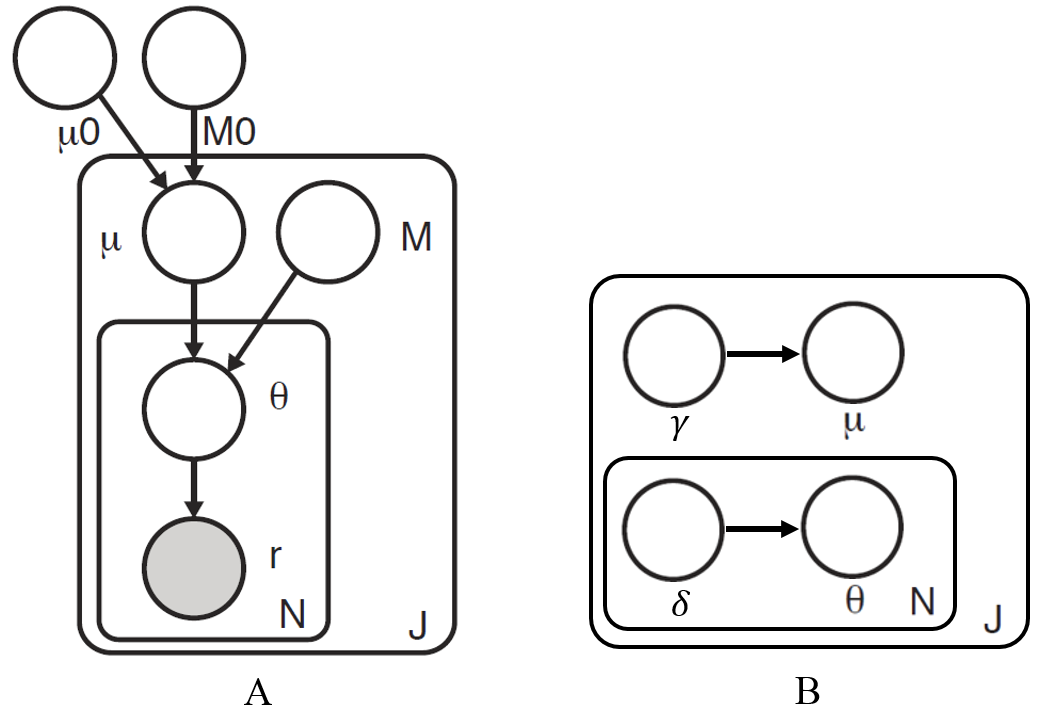
\includegraphics[width=0.5\textwidth]{figs/rvd3_model.png}
\caption{A. Graphical model representation of our Bayesian model.
B. Graphical model representation of the variational distribution used to approximate the posterior.
Observed random variables are shown as shaded nodes and latent random variables are unshaded.
The object of inference for the variational EM algorithm is the joint distribution $p(\mu, \theta|r, n)$.}
\label{tbl:graphical_model}
\end{figure}
The model generative process is as follows:
\begin{enumerate}[noitemsep]
	\item For each location $j$:
	\begin{enumerate}
		\item Draw an error rate $\mu_j \thicksim \text{Beta}(\mu_0, M_0)$
		\item For each replicate $i$:
		\begin{enumerate}
			\item Draw $\theta_{ji} \thicksim \text{Beta}(\mu_j, M_j)$
			\item Draw $r_{ji} | n_{ji} \thicksim \text{Binomial}(\theta_{ji}, n_{ji})$
		\end{enumerate}
	\end{enumerate}
\end{enumerate}

\section{Inference and Hypothesis Testing}
\subsection{Variational Expectation Maximization (EM) Inference}
RVD3 improves RVD2 in the way of deterministic posterior distribution inference.
We developed a non-conjugate variational inference algorithm to approximate the posterior distribution,
\begin{equation}
	p(\mu, \theta | r, n; \phi)  = \frac{ p(\mu, \theta, r | n; \phi) } {p ( r | n; \phi)},
\end{equation}
where the parameters are $\phi \triangleq \{\mu_0, M_0, M\}$.
\subsubsection{Factorization}
We propose the following factorized variational distribution to approximate the true posterior over latent variables $\mu_j$ and $\theta_{ij}$.
Here, $q(\mu_j)$ approximates the variational posterior distribution of $\mu_j$, which represents the local error rate distribution in position $j$ across different replicates;
and $q(\theta_{ij})$ approximates the posterior distribution of $\theta_{ij}$, which is the error rate distribution in position $j$ replicate $i$.
\begin{equation}
  q(\mu, \theta) = q(\mu)q(\theta) = \prod_{j=1}^J q(\mu_{j}) \prod_{i=1}^N q(\theta_{ji}).
  \label{eq:vardist}
\end{equation}

\subsubsection{Evidence Lower Bound (ELBO)}
The log-likelihood of the data is lower-bounded according to Jensen's inequality:
\begin{equation}
\begin{split}
\log p \left( r | \phi \right) &= \log \int_\mu \int_\theta p\left(r,\mu,\theta \right) d\theta d\mu \\
&= \log \int_\mu \int_\theta p\left(r,\mu,\theta \right)\frac{q\left(\mu,\theta \right) }{q\left(\mu,\theta \right) } d\theta d\mu \\
&\geq \int_\mu \int_\theta q\left(\mu,\theta \right) \log \frac{ p\left(r,\mu,\theta \right)}{q\left(\mu,\theta \right)} d\theta d\mu \\
&= E_q \left[ \log p\left(r,\mu,\theta \right)\right] - E_q \left[ \log q\left(\mu,\theta \right)\right] \\
&\triangleq \mathcal{L}(q, \phi).
\end{split}
\end{equation}
where $ \phi= \left( \mu_0, M_0, M \right) $.

The item $\mathcal{L}(q, \phi)$ is the evidence of lower bound (ELBO) of the log-likelihood of the data, which is the sum of $q$-expected complete log-likelihood and the entropy of the variational distribution $q$.
The goal of variational inference is maximizing the ELBO.
Equivalently, $q$ is chosen by minimizing the Kullback-Liebler (KL) divergence between the variational distribution and the true posterior distribution.

\subsubsection{Variational Distributions}
The posterior distribution of $\theta_{ij}$ is a Beta distribution,
\begin{align}
&p(\theta_{ji}|r_{ji},n_{ji},\mu_j,M_j)\\
&\thicksim \text{Beta}(r_{ji}+M_j \mu_j, n_{ji}-r_{ji}+M_j(1-\mu_j)).
\end{align}
Therefore, we propose a Beta distribution with parameter vector $\delta_{ji}$ as variational distribution,
\begin{align}
\theta_{ji} &\thicksim \text{Beta}(\delta_{ji}) \nonumber
\end{align}
%
The posterior distribution of $\mu_j$ is given by its Markov blanket
\begin{align}
p(\mu_j|\theta_{ji},M_j,\mu_0,M_0)\propto p(\mu_j|\mu_0,M_0)p(\theta_{ji}|\mu_j,M_j).
\end{align}
This is not in the form of any known distribution.
Therefore, we propose Beta distribution with parameter vector $\gamma_{ji}$ as a variational distribution to simplify the variational derivation.
\begin{align}
\mu_j &\thicksim \text{Beta}(\gamma_j) \nonumber
\end{align}

\subsubsection{Variational Expectation Maximization (EM) Algorithm}
Variational EM maximizes the ELBO on the true likelihood, by alternating between maximization over $q$ (E-step) and maximization over $\phi$ (M-step).

\begin{algorithm}[h]
  \caption{RVD3 Variational Inference}

  \begin{algorithmic}[1]

  \State Initialize $ q(\theta, \mu) $ and $\hat{\phi}$

  \Repeat

	\Repeat
	
		\For {j = 1 to J}					
			\For {i = 1 to N}				
			\State Optimize $\mathcal{L}(q, \hat{\phi})$ over $q(\theta_{ji}; \delta_{ji}) = \text{Beta} (\delta_{ji})$				
			\EndFor			
		\EndFor
	
		\For {j = 1 to J} 		
			\State Optimize $\mathcal{L}(q, \hat{\phi})$ over $q(\mu_j; \gamma_j) = \text{Beta} (\gamma_j)$			
		\EndFor
	
	\Until{change in $\mathcal{L}(q,\hat{\phi})$ is small}

  \State Set $\hat{\phi} \leftarrow \arg \max\limits_{\phi}
            \mathcal{L}(q,\phi)$
  \Until {change in $\mathcal{L}(q,\hat{\phi})$ is small}

  \end{algorithmic}

\end{algorithm}

\subsection{Posterior Distribution Test}
%%%%%%%%%%%%%%%%%%%%%%%%%%%%%%%%%%%%%%%%%%%%%%%%%%%%%%%%%%%%%%%%%%% Z-test %%%%%%%%%%%%%%%%%%%%%%%%%%%%%%%%%%%%%%%%%%%%%%%%%%%%%%%%%%%%%%%%%%%%%%%%
Variational inference provides variational distributions for $q(\mu_j|r^{control})$ and $q(\mu_j|r^{case})$, which are approximated to the posterior distributions for $p(\mu_j|r^{control})$ and $p(\mu_j|r^{case})$.
We use a $Z$-test based on the Gaussian distribution,

%\begin{equation}
\begin{align}
\label{eq:test}
& \mu_j^{\triangle} = \mu_j|r^{case}-\mu_j|r^{control}\\
& \sigma_j^{\triangle} = \sqrt {var_q{[\mu_j|r^{case}]} + var_q{[\mu_j|r^{control}]}}\\
& Z_j = \frac{\tau - \mu_j^{\triangle}}{{\sigma_j}^{\triangle}}\\
& Pr(Z_j) < \alpha
\end{align}
%\end{equation}

where $\tau$ is a detection threshold and $\alpha$ is a significance level. Here we set $\tau = 0$ and $\alpha = 0.05$.
$\mu_j^{case}$ and $\mu_j^{control}$ are means of distributions.
$var_q{[\mu_j|r^{case}]}$ and  $var_q{[\mu_j|r^{control}]}$ are variances of distributions.
A position is called as a variant when the p-value is less than the significant level $\alpha$.

%%%%%%%%%%%%%%%%%%%%%%%%%%%%%%%%%%%%%%%%%%%%%%%%%%%%%%%%%%%%% Chi-square test %%%%%%%%%%%%%%%%%%%%%%%%%%%%%%%%%%%%%%%%%%%%%%%%%%%%%%%%%%%%%%%%%%%%%%%
A $\chi^2$ goodness-of-fit test for non-uniform base distribution is also used to distinguish a scenario of a true variant from a scenario of a random sequencing error \citep{efron2010large, he2015rvd2}.
By rejecting the null hypothesis that the distribution is uniform, we are able to select variants that represent a true variant in the cell population.

\section{Results}
\subsection{Data Sets}
\subsubsection{Synthetic DNA Sequence Data}
Two random 400bp DNA sequences were synthesized. One sample with 14 loci variants is taken as the case and the other without variants is taken as the control.
Case and control samples were mixed to yield defined VAFs of $0.1\%$, $0.3\%$, $1.0\%$, $10.0\%$, and $100.0\%$.
The details of the experimental protocol are available in \citep{flaherty2011ultrasensitive}.
The synthetic DNA data were downsampled by 10$\times$, 100$\times$, 1,000$\times$, and 10,000$\times$ using Picard.
The final data set contains read pairs for 6 replicates for the control at different VAFs levels.

\subsubsection{Longitudinal Directed Evolution Data}
The longitudinal yeast data comes from three strains of haploid S288c which were grown at $-80^{\circ }\textrm{C}$ for 448 generations under limited-glucose (0.08$\%$).
The Illumina sequencing data are available on NCBI with number SRA054922.
The wild-type ancestral strain GSY1136 was sequenced as a reference.
Aliquots were taken about every 70 generations and sequenced.
The detail of library sequencing is described in \citep{kvitek2013whole, kao2008molecular}.
The aligned BAM files have 266-1046$\times$ coverage.
We used SAMtools -mpileup to convert BAM files to pileup files.
Then we generated depth chart files, which are tab-delimited text files recording the count of the number of nucleotides in columns and genomic positions in rows.
We ran our statistical method on the depth chart files to identify SNVs.

\subsection{Performance on Synthetic DNA Data}
\subsubsection{Comparison of Sensitivity and Specificity}
We compared the performance of our variational algorithm and the MCMC sampling method in the performance of sensitivity and specificity (Table~\ref{tbl:statistics_mcmc_var}).
We used posterior distribution test and $\chi^2$ test to detect variants for a broad range of median read depths and different variant allele frequencies.
The variational algorithm works better than MCMC in sensitivity and specificity in the events when VAF is 0.1\%.
When median read depth is 40000$\times$, the variational algorithm has higher specificity compared with MCMC at events of 0.3\% and 1.0\% VAF with a slight degradation in sensitivity due to false negatives.

% results are under folder \fzhang\Research\rvd3-variational-notebook\results\2015-09-28_Run_rvd3_synthetic_data_set
\begin{table}[h]
\centering
%\vspace{-5pt}
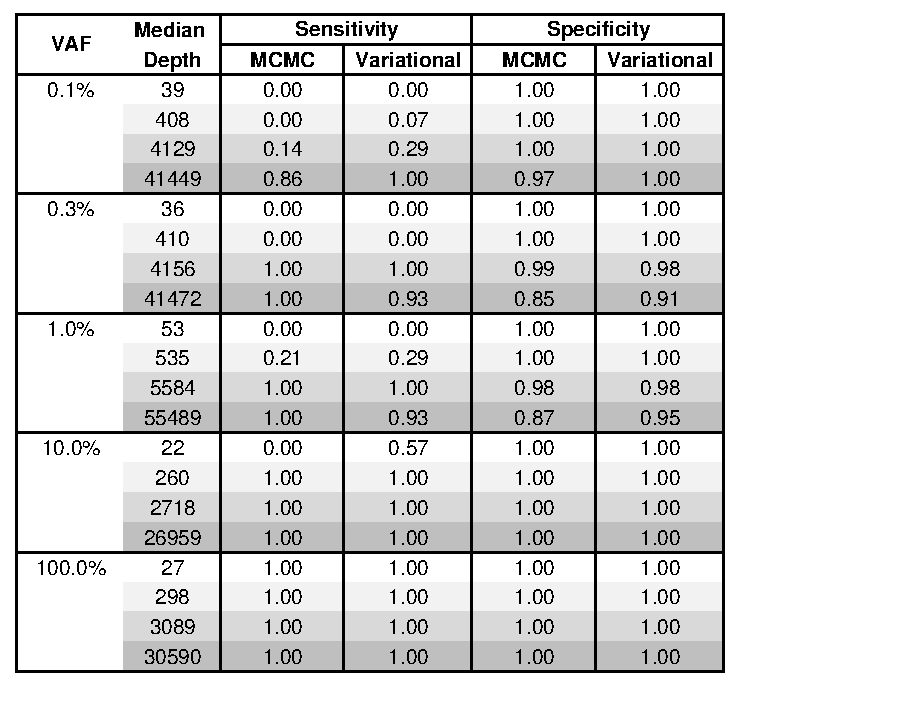
\includegraphics[width=0.8\textwidth]{tables/statistics_mcmc_var.pdf}
\caption{Sensitivity/Specificity comparison of variational algorithm with MCMC on the synthetic DNA data set.}
%\vspace{-10pt}
\label{tbl:statistics_mcmc_var}
\end{table}

\subsubsection{Comparison of Approximated Posterior Distribution}
We showed the approximated posterior distribution of the variational algorithm and exact samples of MCMC.
The variational and MCMC methods both identify all the variants when VAF is 10.0\% and 100.0\%.
One variant position 85 is taken as an example to show the comparison of approximated posteriors (Figure~\ref{tbl:compare1}).
The variational method calls some false positive positions when VAFs are 0.1\% and 0.3\% for low median read depth (30$\times$ and 400$\times$) without a $\chi^2$ test.
Here, a non-mutated position that is called by variational while not called by MCMC (Figure~\ref{tbl:compare2}).
The variance of MCMC posterior distribution is wider than that of the variational method. %, so that variational called it as a variant by a significant difference test.
To increase the specificity of our variational algorithm, the $\chi^2$ test helps to filter this false positive position on a multinomial distribution over the non-reference bases.
We tested 10 random initial posterior distributions and the approximated posterior distributions are the same.
It is also noticeable that the shape of the variational distributions using Beta distribution is exactly displayed as a Gaussian distribution.

% results are under folder \fzhang\Research\rvd3-variational-notebook\results\2015-10-14_Plot_mcmc_mu_vs_variational_mu
\begin{figure}[htbp]
\centering
%\vspace{-10pt}
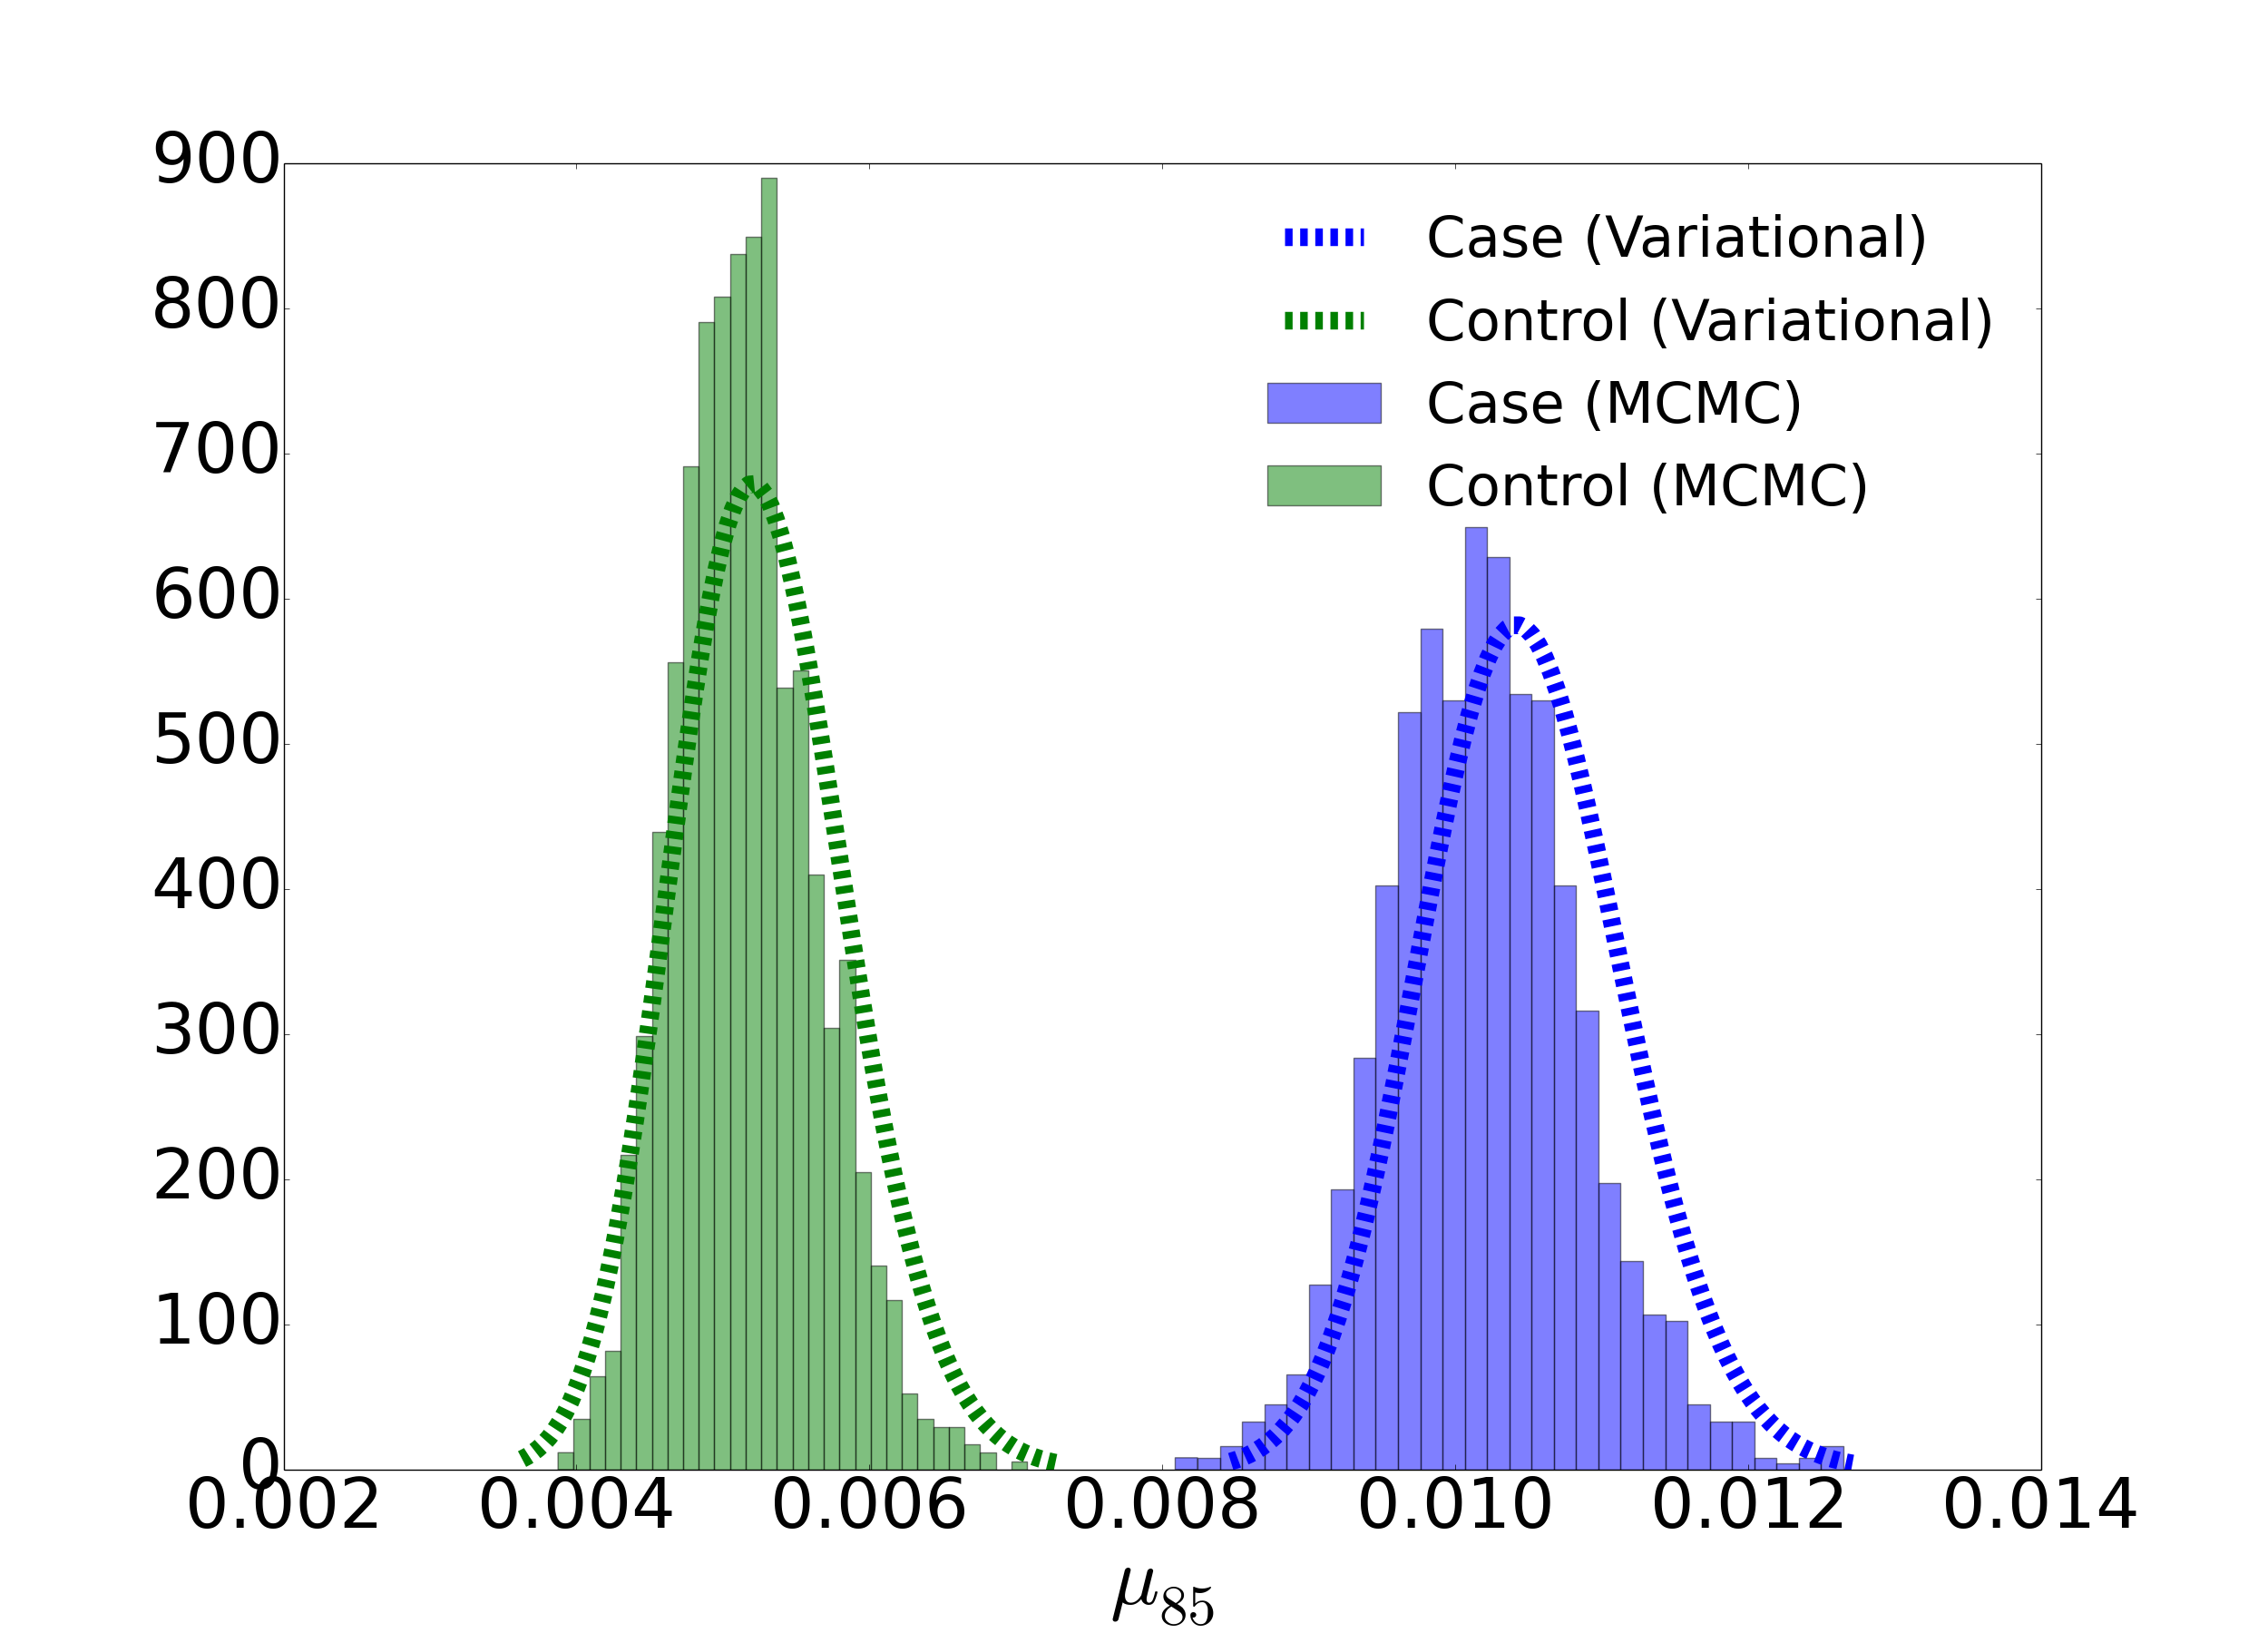
\includegraphics[width=0.7\textwidth]{figs/position_85_5584_mcmc_vs_var_mu_fig1.png}
\caption{Approximated posterior distribution by the variational algorithm and MCMC methods on a true variant position 85 when the median read depth is 5584$\times$.}
%\vspace{-10pt}
\label{tbl:compare1}
\end{figure}

\begin{figure}[htbp]
\centering
%\vspace{-10pt}
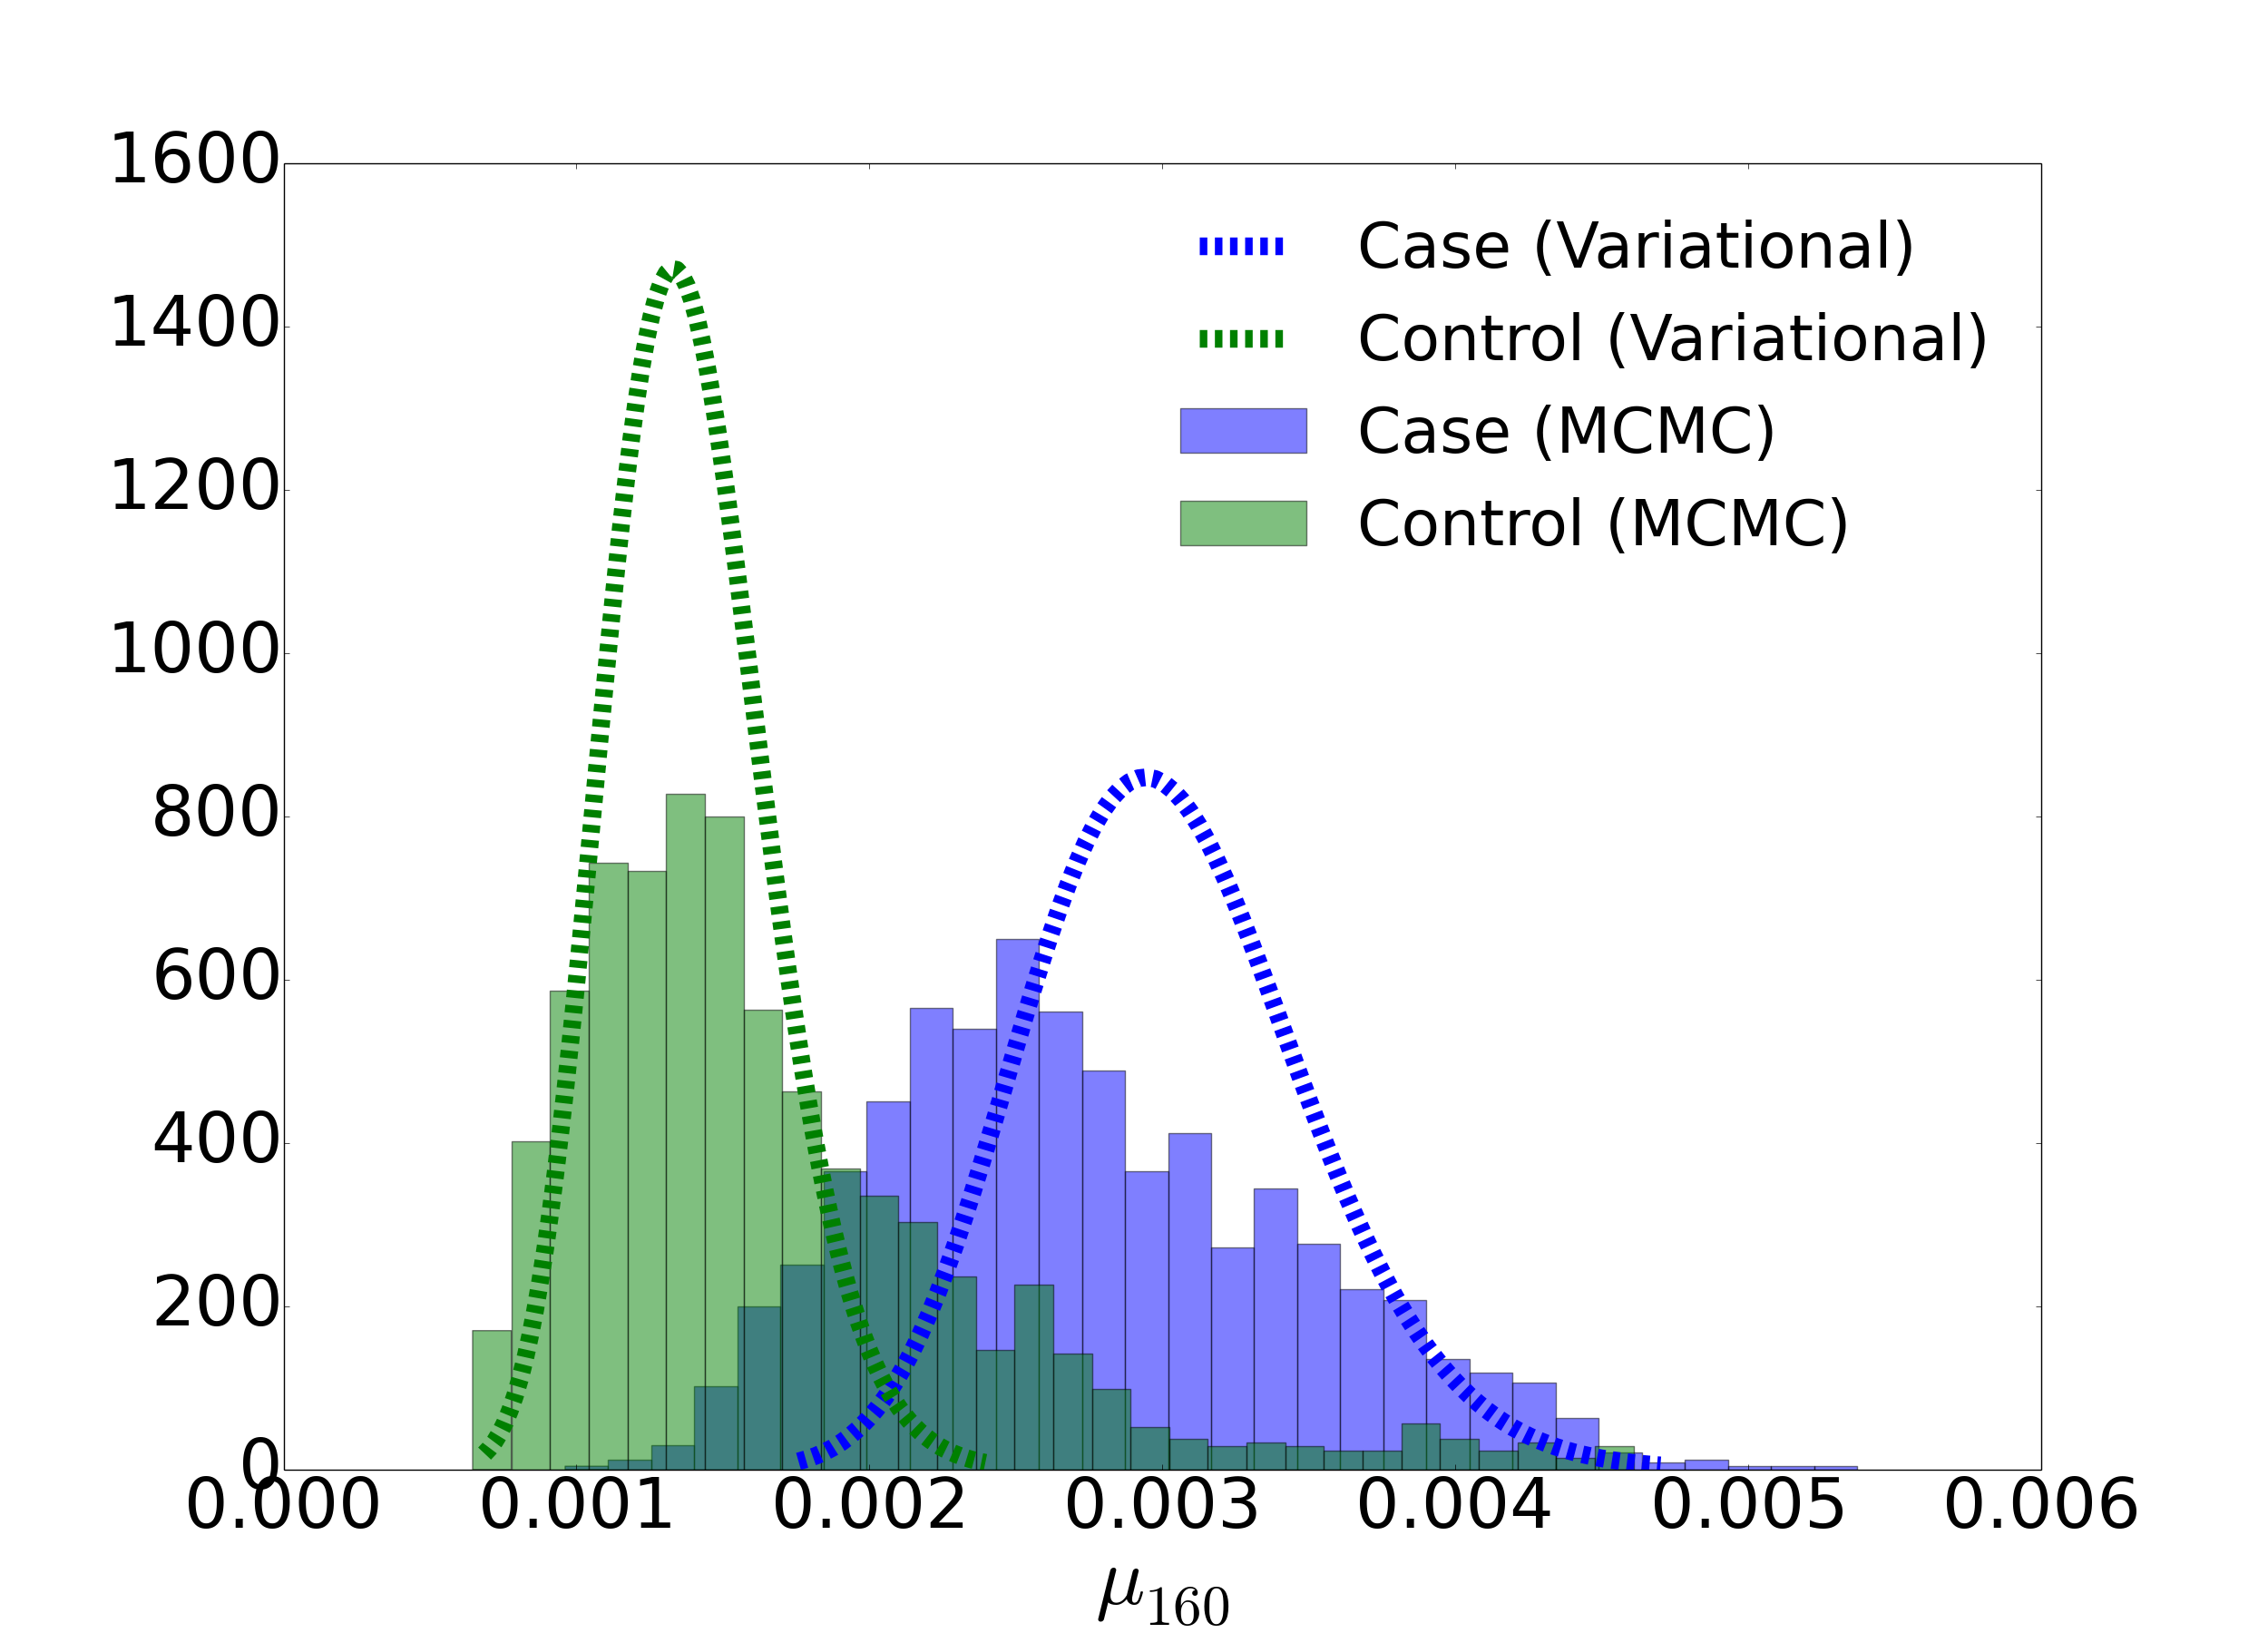
\includegraphics[width=0.7\textwidth]{figs/position_160_410_mcmc_vs_var_mu_fig2.png}
\caption{Approximated posterior distribution by the variational algorithm and MCMC methods on a false variant position 160 when the median read depth is 410$\times$.}
%\vspace{-5pt}
\label{tbl:compare2}
\end{figure}

\subsubsection{Comparison to the State-of-the-Art Approaches}
We compared the performance of our variational algorithm (RVD3) with the state-of-the-art variant detection approaches using synthetic DNA data set (Table~\ref{tbl:character_all}).
Among all of the methods compared, RVD3 shows a high sensitivity and specificity for a broad range of read depths and variant allele frequencies.
RVD3 also performs with higher specificity than all the other tested methods at very low VAF (0.1\%).
RVD3 has a slightly lower specificity than RVD2 only when the median read depth is 4156$\times$ at 0.3\% VAF, and a slightly lower sensitivity than RVD2 only when the median read depth is 41472$\times$ at 0.3\% VAF, and a median read depth of 55489$\times$ at 1.0\%.
He, $\mathit{et} \mathit{al}$, states the performance of other approaches in \citep{he2015rvd2}.

\begin{table*}[htbp]
\centering
%\vspace{-10pt}
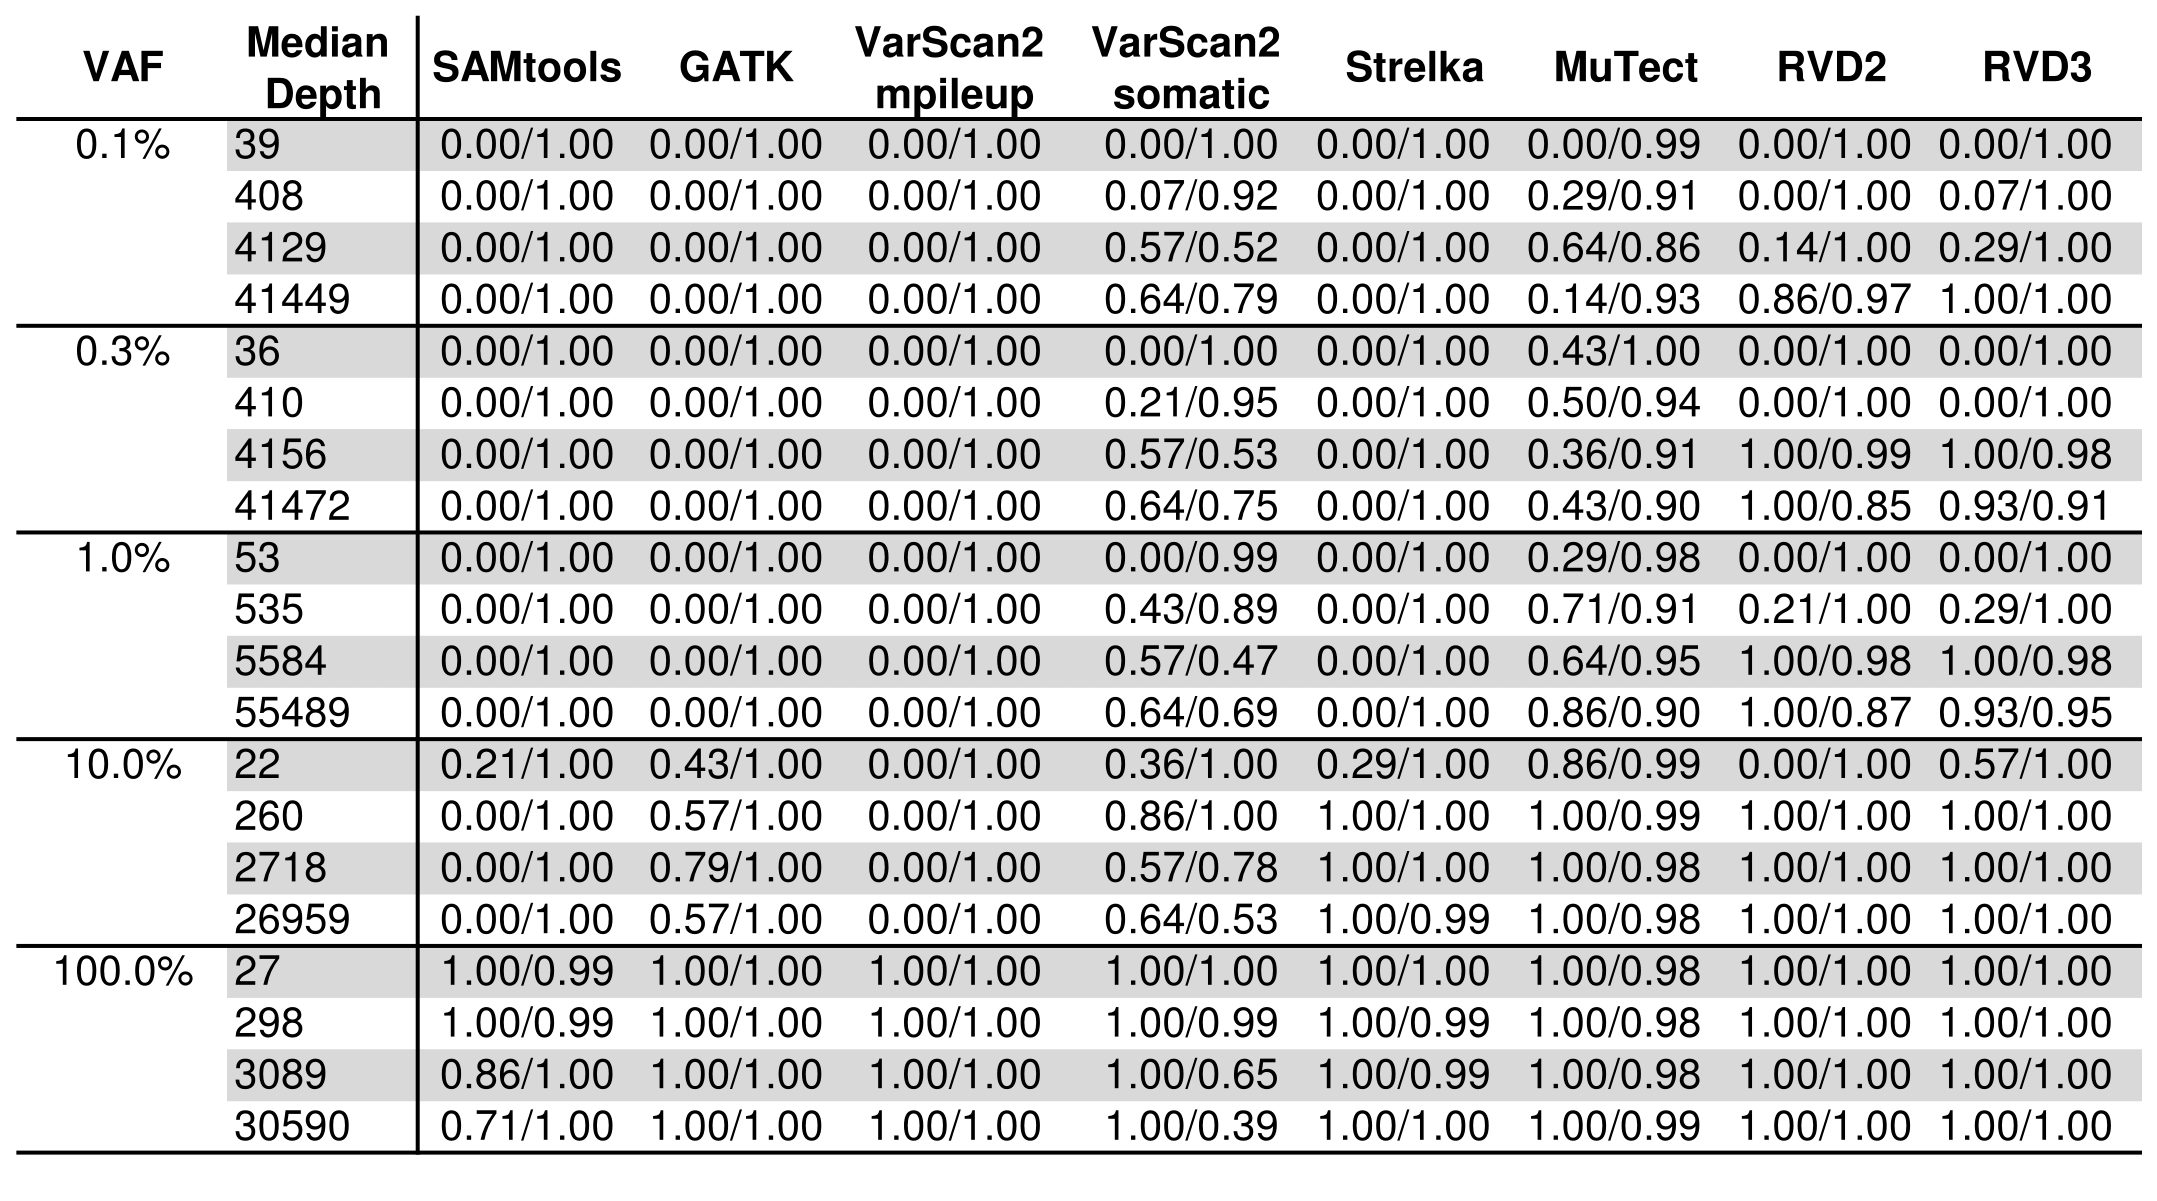
\includegraphics[width=1.0\textwidth]{tables/character_all.png}
\caption{Sensitivity/Specificity comparison of our variational algorithm (RVD3) with other variant detection approaches on synthetic DNA data.}
\vspace{-5pt}
\label{tbl:character_all}
\end{table*}

\subsubsection{Comparison of Timing}
%%%%%%%%%%%%%%%%%%%%%%%%%%%%%%%%%%%%%%%%%%%%%%%%%%%%%%%%%%%%%%% Timing comparison %%%%%%%%%%%%%%%%%%%%%%%%%%%%%%%%%%%%%%%%%%%%%%%%%%%%%%%%%%%%%%%
Time for approximating variational posterior distribution is increased by expanding the length of region of interest and the median read depth (Figure~\ref{tbl:timing_mcmc_var}).
Our variational algorithm works faster than MCMC at low median read depths (27$\times$ and 298$\times$), while it shows the opposite at high median read depths (3089$\times$ and 30590$\times$).

% results are under folder \fzhang\Research\rvd3-variational-notebook\results\2015-10-15_Plot_time_vs_region_length_rvd3_synthetic_data
\begin{figure}[h]
\centering
%\vspace{-5pt}
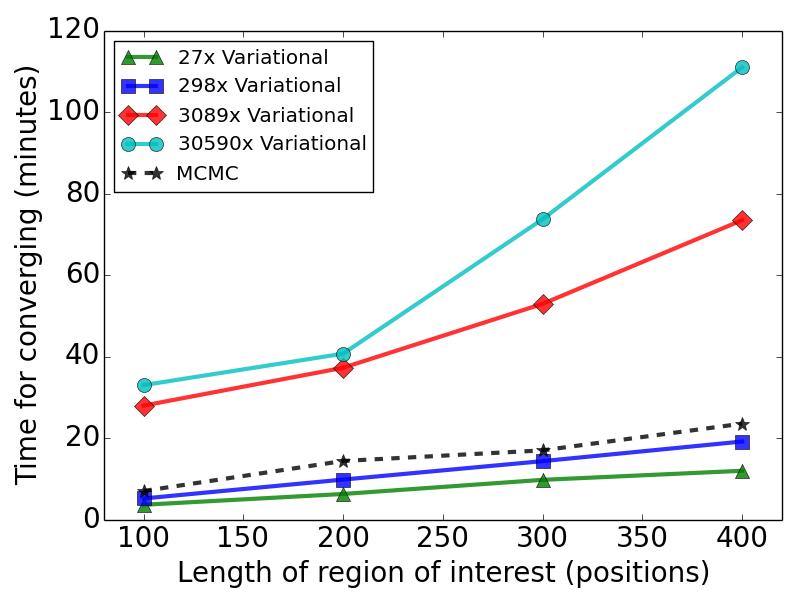
\includegraphics[width=0.6\textwidth]{figs/timing_var_mcmc.png}
\caption{Timing figure for our variational algorithm and MCMC sampling.
Parallel computational cores (60 processers) are used to estimate the model on the synthetic data set.}
%\vspace{-10pt}
\label{tbl:timing_mcmc_var}
\end{figure}

%%%%%%%%%%%%%%%%%%%%%%%%%%%%%%%%%%%%%%%%%%%%%%%%%%%%%%%%%%% Timing profile of variational %%%%%%%%%%%%%%%%%%%%%%%%%%%%%%%%%%%%%%%%%%%%%%%%%%%%%%%%%%
The timing profile for each part of our variational algorithm when median read depth is 3089$\times$ is also shown in Table~\ref{tbl:timing_profile_all}.
Optimizing $\gamma$ function in E-step and optimizing $M$ in M-step takes more than 95\% of the time of one variational iteration in a test of a single processor, as such a time consuming integration is needed.

% results are under folder \fzhang\Research\rvd3-variational-notebook\results\2015-10-21_Timing_profile_rvd3_program
\begin{table*}[htbp]
\centering
\vspace{10pt}
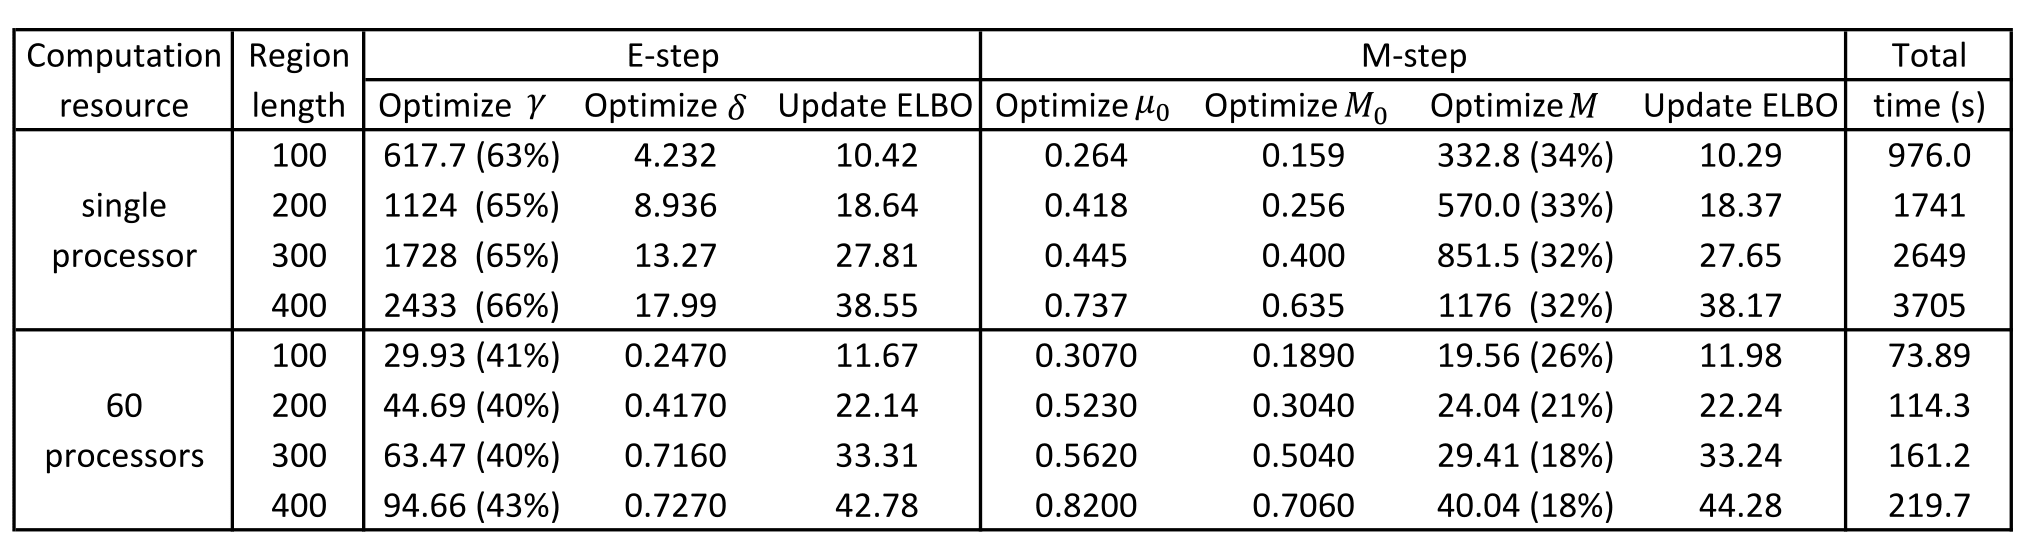
\includegraphics[width=1.0\textwidth]{tables/time_3089X_all_update.png}
\caption{Timing profile of 4 significant figures for one iteration of variational algorithm when median read depth is 3089$\times$.
Single and multiple processors are both tested to estimate timing. Time for optimizing $\gamma$ function in E-step and optimizing $M$ in M-step is highlighted in percentage.}
%\vspace{-10pt}
\label{tbl:timing_profile_all}
\end{table*}

\subsection{Variant Detection on the Longitudinal Directed Evolution Data}
%%%%%%%%%%%%%%%%%%%%%%%%%%%%%%%%%%%%%%%%%%%%%%%%%%%% Generally describe detected variants %%%%%%%%%%%%%%%%%%%%%%%%%%%%%%%%%%%%%%%%%%%%%%%%%%%%%%%%%%%%%%%%%%%
We applied our method on the MTH1 gene, region of 1302bp, on Chr04:1014401-1015702, which is the most frequently observed mutated gene \citep{kvitek2013whole}.
Our method detected the same variants that were found by Kvitek and Sherlock, 2013 and marked as blue in Table~\ref{tbl:mutations}.
Additionally, we detected 81 novel variants in 8 timepoints that the original publication missed.
In Table~\ref{tbl:mutations}, G7 is the baseline VAF as the control sample when comparing with G70, G133, G266, G322, G385, and G448 in the respective hypotheses testing.
The corresponding VAFs of called variants in different time points are given by the estimation of the latent variable $\mu_j$.

%%%%%%%%%%%%%%%%%%%%%%%%%%%%%%%%%%%%%%%%%%%%%%%%%%%% Beneficial variant and early identification %%%%%%%%%%%%%%%%%%%%%%%%%%%%%%%%%%%%%%%%%%%%%%%%%%%%%%%%%%%%
All of these variants, except variant in position 1014740, decrease in VAF following a maximum and eventually become extinct.
Allele on position 1014740 is a beneficial variant that arises in frequency to 99.603\% at generation 448 within a constant glucose-limited environment.
Moreover, we identified the first emergence of this beneficial mutation as early as 0.522\% in generation 133.
Table~\ref{tbl:mutations} shows that we are able to detect many variants ($<$ 1.0\%) early in the evolutionary time course.
Furthermore, we detected a variant on position 1015666 at generation 70 as 0.091\%, which is less than a 0.1\% fraction.

%%%%%%%%%%%%%%%%%%%%%%%%%%%%%%%%%%%%%%%%%%%%%%%%%%%%%%%%%%%%% Concomitant variants  %%%%%%%%%%%%%%%%%%%%%%%%%%%%%%%%%%%%%%%%%%%%%%%%%%%%%%%%%%%%%%%%%%%%%%%%%
We also identified a pair of concomitant variants, Chr04:1014740 in gene MTH1 and Chr12:200286 in gene ADE16, that increase in VAF together in time (Figure~\ref{tbl:concomitant} A).
The venn diagram shows the logical relation between the concomitant variants (Figure~\ref{tbl:concomitant} B).
In generation 448, the minimum intersection of the concomitant variants in gene MTH1 and gene ADE16 is 98.49\%.
In this pair of genes, gene MTH1 is a negative regulator of the glucose-sensing signal transduction pathway, and gene ADE16 is an enzyme of $\mathit{de novo}$ purine biosynthesis.
Glucose sensing inducts gene expression to help yeast receive necessary nutrients, which could be a reason for this pair of genes to mutate together \citep{johnston1999feasting}.

% results are under folder \fzhang\Research\rvd3-variational-notebook\results\2016-01-12_Run_rvd3_Dan_data_regions
\begin{table*}[htbp]
\centering
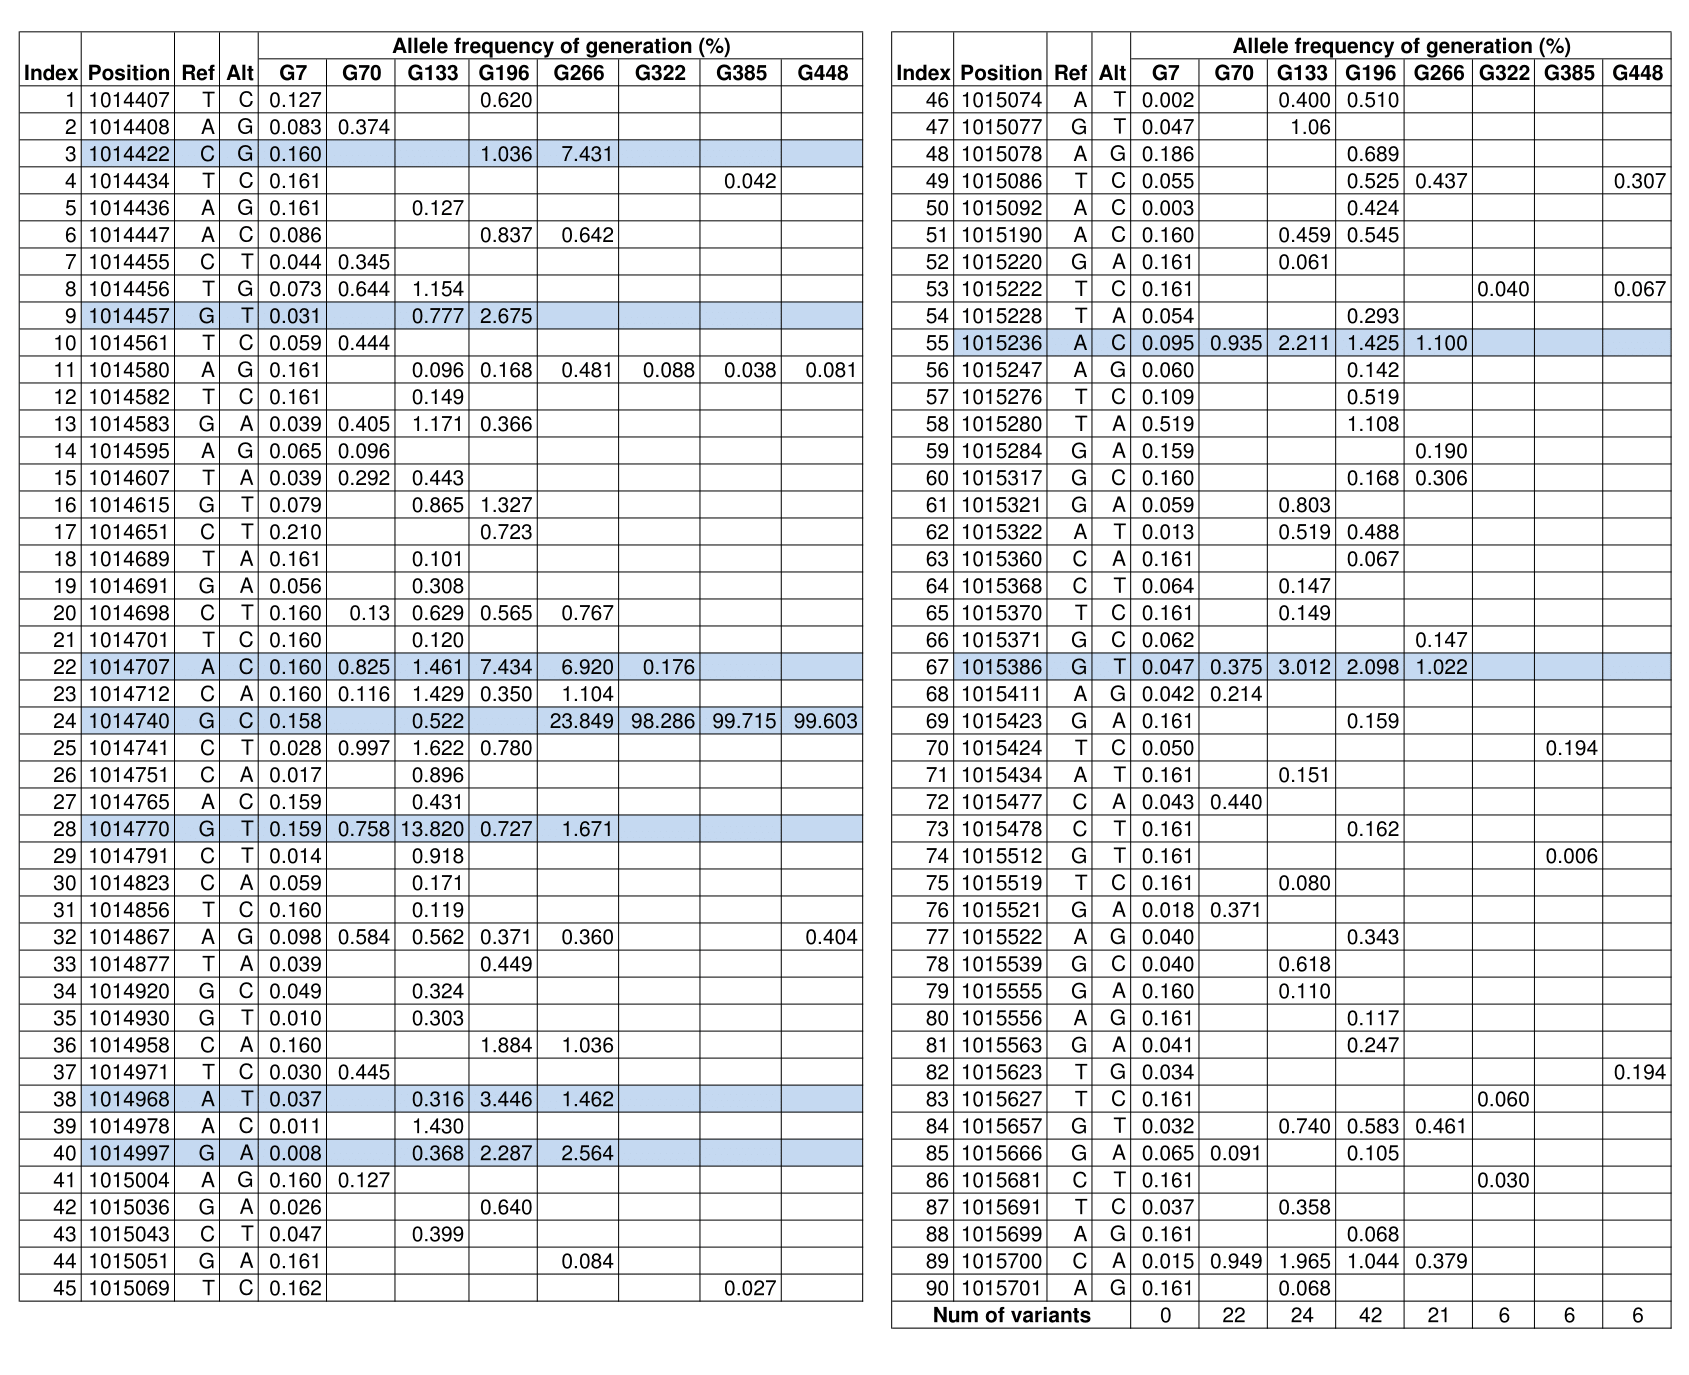
\includegraphics[width=1.0\textwidth]{tables/mutations_MTH1.png}
\caption{Identified variants and corresponding VAF in gene MTH1 on Chromosome 4.
The blank means no variant is identified in one event.
Positions marked as blue were also identified by Kvitek, 2013.
Other positions are 81 novel identified variants in 8 timepoints.}
\label{tbl:mutations}
\end{table*}
\begin{figure}[h]
\centering
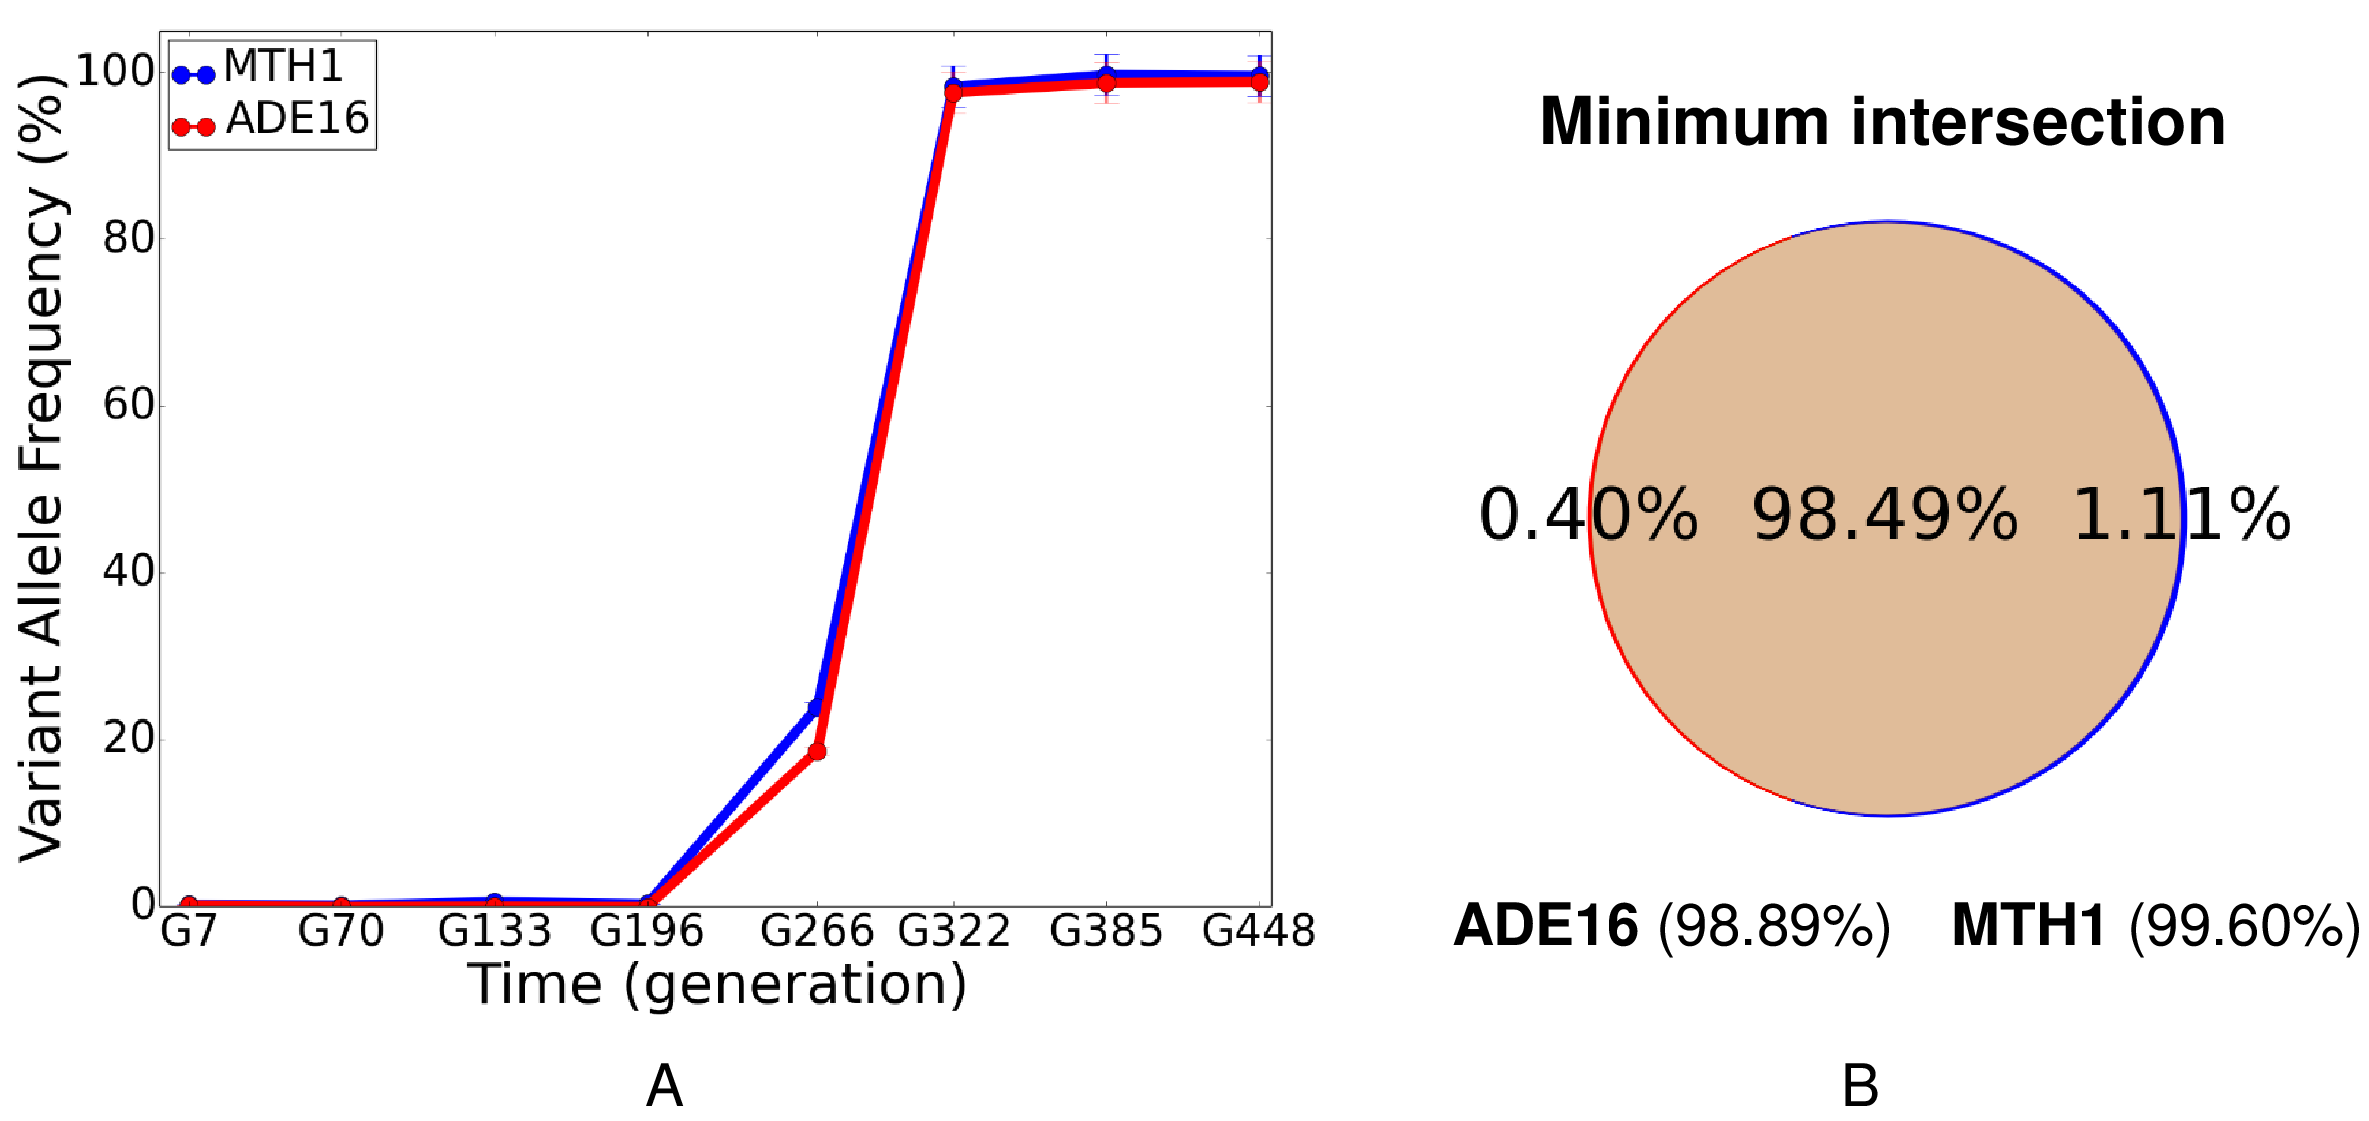
\includegraphics[width=0.8\textwidth]{figs/concomitant_figure.png}
\caption{A. The VAF trend of concomitant variants in gene MTH1 and ADE16.
The 95\% Bayesian credible interval are shown.
B. The venn diagram shows the logical relation between the concomitant variants in generation 448.}
%\vspace{-10pt}
\label{tbl:concomitant}
\end{figure}

\section{Discussion}
%%%%%%%%%%%%%%%%%%%%%%%%%%%%%%%%%%%%%%%%%%%%%%%%%%%%%%%%%%%%% Brief summary of RVD3 %%%%%%%%%%%%%%%%%%%%%%%%%%%%%%%%%%%%%%%%%%%%%%%%%%%%%%%%%%%%%%%%%%%
In this article, we propose a Bayesian statistical model, called RVD3, to estimate the VAF by approximating posterior distributions for latent variables.
We derived a variational expectation maximization algorithm to calculate the intractable integration of our Bayesian model.
Our results shows that RVD3
(i) is able to identify rare variants at a 0.1\% fraction level with improved sensitivity and specificity in comparison to a MCMC sampling algorithm;
(ii) has a higher specificity in comparison with some state-of-the-art algorithms in a broad range of mixed samples;
and (iii) detects SNVs early in the evolutionary time course, as well as track the VAF in a longitudinal data set.

%%%%%%%%%%%%%%%%%%%%%%%%%%%%%%%%%%%%%%%%% Potential problems of variational EM and alternative strategies %%%%%%%%%%%%%%%%%%%%%%%%%%%%%%%%%%%%%%%%%%%%%%
However, the application of RVD3 on an interested gene region suggests that our variational EM algorithm yields a accurate and efficient result.
It is possible that the Beta variational distribution we have selected to address the non-conjugate prior issue will not yield the speed improvements we expect.
In that event, we will instead use a straightforward interpolation scheme to compute the necessary integral for the expectation step.
The Beta function in the integral kernel is relatively smooth and has a bounded domain.
This favorable property can be leveraged to implement a cubic spline interpolation method to approximate the necessary integral \citep{mckinley1998cubic}.
Another strategy is to consider a Laplace approximation for the proposal variational distribution, as we and others have done previously \citep{saddiki2014glad, wang2013variational}.

As a local optimization methodology, variational EM is possible to fall in a local maximum of the variational function.
It could be that the accuracy is still not sufficient to identify variants with statistical confidence.
If sot, we will generate different random initialized parameters to restart the algorithm.
We can also consider using the RVD2 model for more accurate posterior approximation, which is implemented by MCMC sampling.
MCMC is computationally slower, but is easily deployed to multiple computational cores in parallel.
Thus, we will be able to analyze the sequencing data using Amazon Elastic Compute Cloud (EC2) resource, which will increase computation efficiency.

%%%%%%%%%%%%%%%%%%%%%%%%%%%%%%%%%%%%%%%%%%%%%%%%%%%%%%%%%%%%%% Future work %%%%%%%%%%%%%%%%%%%%%%%%%%%%%%%%%%%%%%%%%%%%%%%%%%%%%%%%%%%%%%%%%%%%%%%%%%%%%%
RVD3 discovers many novel variants in the application of an interested region of the longitudinal yeast data set.
These discovered variants drive us to extend our statistical method to the whole genome, whole population yeast sequence data with guaranteed accuracy and efficiency.
By doing this, we can uncover the dynamics of arising variants at the genome-wide scale to show the genetic basis of clonal interference.
Our method is also can be extended to study drug resistance by characterizing tumor heterogeneity in targeted anti-cancer chemotherapy samples.
We will be able to find the causative variants that lead to drug resistance and understand the causes of resistance at the single nucleotide level.

\section*{Acknowledgments}
Funding:


\appendix

\bibliographystyle{named}
\bibliography{ref}

\end{document}